\documentclass[12pt]{article}
\usepackage[a4paper,margin=3cm]{geometry}
\usepackage{graphics}
\usepackage{underscore}
\usepackage{fancyvrb}
\usepackage{url}

\fvset{xleftmargin=1cm}
\DefineShortVerb{\|}

\newcommand{\F}{Figure~}

\title{Executing ARM code in HOL.}
\author{}
\date{}

\begin{document}
\maketitle

\subsection*{Initial Setup}

\subsubsection*{Binutils}

ARM code is generated using the GNU assembler; this can be downloaded from
\begin{quote}
\url{http://ftp.gnu.org/gnu/binutils/}
\end{quote}
By default the assembler will generate native code.  To configure it to generate ARM code, one must enter:
\begin{Verbatim}
./configure --prefix=$BINHOME --target=arm-coff
make
make install
\end{Verbatim}
where \url{BINHOME} is the directory where you wish to install the \textsf{binutils} package.
The file \url{$HOLDIR/example/arm6/testScript.sml} should then be edited, setting the  \url{BINUTILS} variable to correspond with \url{BINHOME}.

\subsubsection*{Smltk}

The front-end uses \textsf{sml_tk}, which can be downloaded from
\begin{quote}
\url{http://www.informatik.uni-bremen.de/~cxl/sml_tk/}
\end{quote}
This package uses Moscow ML's dynamic libraries, so at the moment, it will not work for MacOS X.  You will also need a working version of Tcl/Tk.  In order to work with HOL, a couple of edits need to be made to the file \url{$TKHOME/src/export.sml} (where \url{TKHOME} the directory where you put \textsf{sml_tk}).  Line 159 should become
\begin{Verbatim}
val +++ : AnnoText * AnnoText -> AnnoText
\end{Verbatim}
and line 398 needs to be commented out.  It is also necessary to edit the file \url{$HOLDIR/tools/unquote-init.sml}.  Line 19 should become
\begin{Verbatim}
end handle Io _ => false
\end{Verbatim}

\fvset{xleftmargin=5mm}

\subsection*{Running the Simulator}

To start the front-end:
\begin{enumerate}
\item Change directory to \url{$HOLDIR/examples/arm6}
\item Do a |Holmake| -- the make will eventually fail on the file \url{testScript.sml}
\item Start an interactive session with
\begin{Verbatim}
hol -I $TKHOME/src
\end{Verbatim}
\item Enter
\begin{Verbatim}
app load ["Unix","listLib","compLib", "io_onestepTheory",
   "armLib", "coreLib", "disassemblerLib", "patriciaLib"];
\end{Verbatim}
followed by
\begin{Verbatim}
use "testScript.sml";
\end{Verbatim}
and then
\begin{Verbatim}
go();
\end{Verbatim}
\end{enumerate}
Two windows will appear: one enables you to view and edit the current state of the memory; the other window lets you edit the ARM registers and start a run -- see \F\ref{reg:fig}.   One can specify the number of cycles to be executed -- if this is left blank, execution will continue until an \emph{undefined} instruction exception is taken.  The output of the function |go| is a list of theorems; these give the state and output of the program for each cycle.
\begin{figure}
\begin{center}
\scalebox{.5}{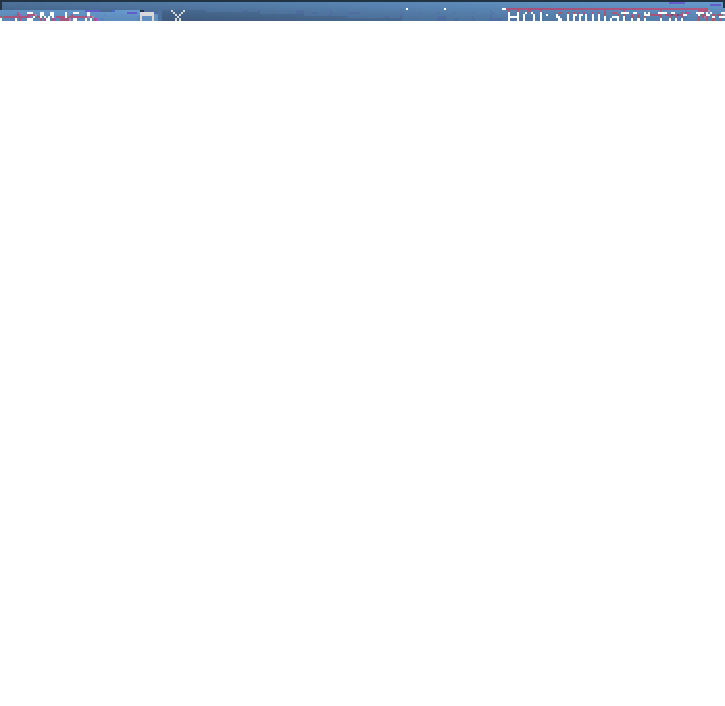
\includegraphics{reg.pdf}}
\caption{Register viewer.}
\label{reg:fig}
\end{center}
\end{figure}

\subsection*{ARM Assembly}

The function |assemble : num -> string list -> unit| can be used to load ARM code into memory.  For example, the call
\begin{Verbatim}
assemble Arbnum.zero
  ["movs pc, #32",
   "label: b label",
   "movs pc, r14",
   "subs pc, r14, #4",
   "subs pc, r14, #8",
   "movs pc, r14",
   "subs pc, r14, #4",
   "subs pc, r14, #4"]
\end{Verbatim}
is used to load the exception handler at the start of the memory.  The |assemble| function calls the GNU assembler -- if the assembler fails to create a binary, the output from the assembler will be printed.  The created object file uses big-endian byte ordering.

\subsection*{The Memory}

The memory is an ML value, |memory|.  The first eight instructions in memory are used to handle exceptions -- in the rudimentary default program above: the \emph{reset} handler simply exits to location |0x20|; the \emph{undefined instruction} handler loops indefinitely; and all of the other handlers return to the \emph{link register} address. The memory is initially full of undefined instructions, so ``running off the end'' of a block of code will cause termination.

The viewer (see \F\ref{mem:fig}) enables one to examine blocks of memory.  One can: view a block (with a double click); wipe blocks (fill them with undefined instructions); load data from, or save data to, a binary file; and edit a single memory line (with a double click).
\begin{figure}
\begin{center}
\scalebox{.5}{
\includegraphics{mem.pdf}}
\caption{Memory viewer.}
\label{mem:fig}
\end{center}
\end{figure}

To run a program, the machine code must be loaded into memory, together with any initial data.  One can use the |assemble| function (see above) and four other ML functions:
\begin{Verbatim}
mem_read : bool option -> num -> num
mem_write : bool -> num -> num -> unit
load_data : string -> int -> num -> unit
save_data : string -> num -> num -> bool -> unit
\end{Verbatim}
The functions |mem_read| and |mem_write| enable one to access a single memory address:
\begin{center}
  \begin{tabular}{@{} ll @{}}
    |mem_read NONE addr| & read a word from |addr| (aligned) \\ 
    |mem_read (SOME false) addr| & read a word  (rotating if not aligned) \\ 
    |mem_read (SOME true) addr| & read a byte from |addr| \\[4pt]
    |mem_write false addr data| & write a word to |addr| (aligned) \\ 
    |mem_write true addr data| & write a byte to |addr| \\
  \end{tabular}
\end{center}
The functions |load_data| and |save_data| are used to read a write chunks of memory to a binary file:
\begin{center}
  \begin{tabular}{@{} lp{70mm} @{}}
    |load_data fname offset addr| & reads from the file |fname| (skipping over |offset| bytes) and stores the data in the memory starting from location |addr|.  (Uses big-endian byte ordering.) \\[4pt]
    |save_data fname start finish le| & saves bytes from |start| to |finish| in the file |fname|.  If |le| is |true| then little-endian ordering is used, otherwise it is big-endian.  \\
  \end{tabular}
\end{center}
In ML one can also create a binary file from a list of bytes using |BinIO.output| and |Word8Vector.fromList|.

\subsection*{The Registers}

The register editor (see \F\ref{reg:fig}) is used to set the initial state of the ARM registers.  One can only enter numeric (decimal) values for registers -- any other entry will be treated as a zero.  The ``exception'' field determines whether the execution starts with an exception call.

\subsection*{The Trace}

Once execution is started, the HOL session will display the time taken to execute each instruction; when the program terminates an execution trace viewer opens (see \F\ref{trace:fig}) and the memory viewer will be updated to show the final state of the memory.  A slider at the bottom of the trace viewer is used to select the cycle.  The ``opcode'' box contains the next instruction to be executed, provided that the current ``exception'' is |software|.\footnote{Although the execution can start with any exception (by default starting with a reset), only \emph{undefined instruction} exceptions can occur at run-time i.e. the ``interrupt'' input is always \texttt{NONE}.  Support might be added later for producing traces with, for example, data aborts and interrupts.}  The ``fetch'' box shows the instruction that is fetched from memory -- the ``data-in'' and ``data-out'' boxes show all other memory requests and input.  Two boxes are used to display the current state of the general purpose and program status registers.
\begin{figure}
\begin{center}
\scalebox{.5}{
\includegraphics{trace.pdf}}
\caption{Execution trace.}
\label{trace:fig}
\end{center}
\end{figure}

\end{document}
